\documentclass{article}
\usepackage{tikz}
\usepackage{amsmath}
\usepackage{graphicx}
\usetikzlibrary{decorations.pathmorphing, arrows.meta, positioning, calc, fit, backgrounds}

\begin{document}

\title{Analysis of a Doubly Spread Channel}
\author{}
\date{\today}

\maketitle

\section{Theoretical Framework}
The theoretical framework defines a \textbf{Doubly Spread Channel} \cite{stojanovic1996recent, preisig2007acoustic} as one driven by two coupled mechanisms: \textbf{Source Kinematics (Heave)} and \textbf{Dynamic Boundary Interaction (Micro-Multipath)}.

\section{Source on the surface}
\subsection{Schematic Diagram}
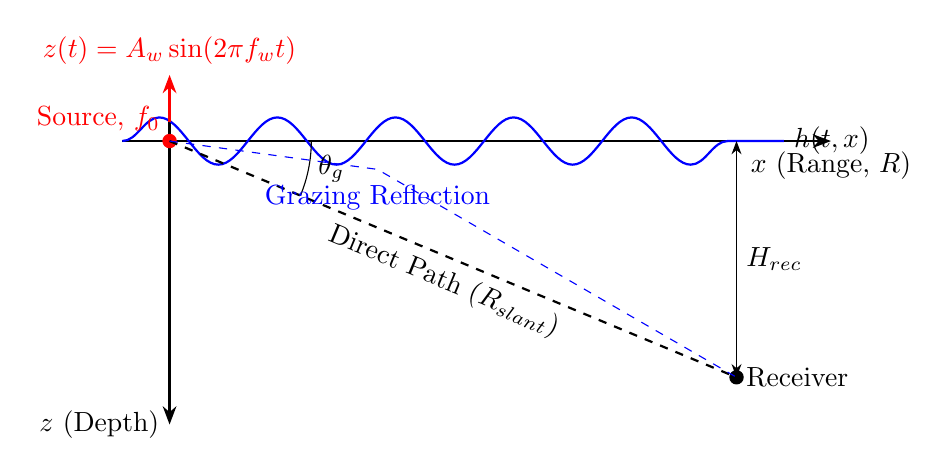
\begin{tikzpicture}[scale=1.2, >=Stealth]

    % Define variables/coordinates
    \def\Range{6}
    \def\Hrec{-2.5}
    
    % Draw axes
    \draw[->, thick] (0, 0.5) -- (0, \Hrec - 0.5) node[left] {$z$ (Depth)};
    \draw[->, thick] (-0.5, 0) -- (\Range + 1, 0) node[below] {$x$ (Range, $R$)};
    
    % Draw rough ocean surface
    \draw[blue, thick, decoration={snake, amplitude=3mm, segment length=15mm}, decorate] 
        (-0.5, 0) -- (\Range + 0.5, 0) node[right, text=black] {$h(t, x)$};
        
    % Source Vessel
    \filldraw[red] (0,0) circle (2pt) node[above left] {Source, $f_0$};
    \draw[->, red, thick] (0, 0.2) -- (0, 0.7) node[above] {$z(t) = A_w \sin(2\pi f_w t)$};
    
    % Receiver
    \filldraw[black] (\Range, \Hrec) circle (2pt) node[right] {Receiver};
    
    % Direct path and angle
    \draw[dashed, thick] (0,0) -- (\Range, \Hrec) node[midway, sloped, below] {Direct Path ($R_{slant}$)};
    \draw (1.5, 0) arc (0:{-atan(2.5/6)}:1.5) node[midway, right] {$\theta_g$};
    
    % Surface interaction path (Shadowing example)
    \draw[blue, dashed] (0,0) -- (2.2, -0.3) -- (\Range, \Hrec);
    \node[blue, align=center] at (2.2, -0.6) {Grazing Reflection};
    
    % Annotate Depth and Range
    \draw[<->] (\Range, 0) -- (\Range, \Hrec) node[midway, right] {$H_{rec}$};
    
\end{tikzpicture}

\subsection{Physical \& Mathematical Breakdown}

\subsubsection{The Grazing Angle}
The grazing angle $\theta_g$ is the angle between the direct acoustic path and the horizontal at the point of reflection. It is given by:
\begin{equation}
\theta_g = \arctan \left( \frac{H_{rec} - H_{src}}{R} \right)
\end{equation}
Because the source is on the surface ($H_{src} \approx 0$) and the range is long ($R \gg H_{rec}$), the grazing angle $\theta_g$ approaches $0^\circ$.
For example, in a setup where the receiver is at 20m depth and the source is 1km away on the surface, $\theta_g \approx 1.15^\circ$.
\subsubsection{The Transmitted Signal: Source Kinematics}
A theoretical underwater acoustic source emits a monochromatic pressure wave $p(t)$ at a fundamental frequency $f_0$:
\begin{align}
p(t) &= P_0 \cos(2\pi f_0 t)
\intertext{Since a surface vessel is physically coupled to the ocean surface, it undergoes vertical heave motion. We approximate the dominant ocean swell as a harmonic oscillation with amplitude $A_w$ and frequency $f_w$:}
z(t) &= A_w \sin(2\pi f_w t)
\intertext{This physical motion acts as a time-varying phase shift on the emitted acoustic wave. The transmitted signal $p_{tx}(t)$ becomes a Phase/Frequency Modulated (FM) signal:}
p_{tx}(t) &= P_0 \cos\left(2\pi f_0 t + \beta \sin(2\pi f_w t)\right)
\intertext{The severity of the phase modulation is defined by $\beta$, which relates the physical heave amplitude to the acoustic wavelength ($\lambda = c/f_0$) and the grazing angle ($\theta_g$):}
\beta &= \frac{2\pi f_0}{c} A_w \cos\theta_g
\intertext{The instantaneous phase $\Phi(t)$ of the transmitted pressure wave is:}
\Phi(t) &= 2\pi f_0 t + \beta \sin(2\pi f_w t) \\
\intertext{Differentiating the phase $\Phi(t)$ with respect to time yields the instantaneous frequency $f_i(t)$, defined as $f(t) = \frac{1}{2\pi} \frac{d\Phi}{dt}$. This is directly analogous to kinematics, where velocity is the time derivative of position ($v(t) = \frac{dx}{dt}$). While a constant phase rate yields a static frequency $f_0$, the heave-induced sinusoidal phase results in a time-varying frequency $f_i(t)$ that physically oscillates around $f_0$:}
f_i(t) &= \frac{1}{2\pi} \frac{d\Phi}{dt} = f_0 + \Delta f \cos(2\pi f_w t) \\
\intertext{where the peak frequency deviation $\Delta f$ is defined as:}
\Delta f &= \beta f_w = \frac{2\pi f_0 f_w}{c} A_w \cos\theta_g
\end{align}

\paragraph{Physical Interpretation of $\beta$:}
The modulation index $\beta = 2\pi (A_w / \lambda) \cos\theta_g$ represents the peak phase shift in radians, governed by two physical balances:
\begin{itemize}
    \item \textbf{Scale Ratio ($A_w / \lambda$):} Compares the physical ship heave amplitude ($A_w$) to the acoustic wavelength ($\lambda$). At high frequencies (short $\lambda$), yielding a large $\beta$ and severe frequency smearing. At low frequencies (long $\lambda$), resulting in a small $\beta$ and minimal smearing.
    \item \textbf{Geometric Projection ($\cos\theta_g$):} Represents the projection of the vertical heave along the acoustic ray path. For shallow grazing angle ($\theta_g \to 0^\circ$), $\cos\theta_g \to 1$, the vertical motion projects fully along the ray path. For a receiver directly above the source ($\theta_g \to 90^\circ$), $\cos\theta_g \to 0$, the vertical motion is perpendicular to the ray direction, resulting in zero path-length modulation and no frequency smearing.
\end{itemize}

\subsubsection*{Spectral Expansion (The Bessel Comb)}
\cite{carlson2001} \\
To analyze the frequency spectrum of the modulated signal, we transition to the frequency domain using the \textbf{Jacobi-Anger expansion}. 

First, we express the time-domain pressure wave $p_{tx}(t)$ as the real part of a complex analytic signal:
\[ p_{tx}(t) = P_0 \text{Re} \left\{ e^{i 2\pi f_0 t} \cdot e^{i \beta \sin(2\pi f_w t)} \right\} \]

Next, we apply the Jacobi-Anger identity, which expands the exponential of a sine function into an infinite series of Bessel-weighted harmonics:
\[ e^{i \beta \sin(\phi)} = \sum_{n=-\infty}^{\infty} J_n(\beta) e^{i n \phi} \]
where $\phi = 2\pi f_w t$. Substituting this expansion back into the pressure wave equation:
\[ p_{tx}(t) = P_0 \text{Re} \left\{ \sum_{n=-\infty}^{\infty} J_n(\beta) e^{i 2\pi (f_0 + n f_w) t} \right\} \]

Taking the real part of each term results in an infinite series of discrete spectral lines (sidebands) spaced at intervals of the ocean wave frequency $f_w$, weighted by Bessel functions of the first kind $J_n$:
\begin{equation}
p_{tx}(t) = P_0 \sum_{n=-\infty}^{\infty} J_n(\beta) \cos\left( 2\pi (f_0 + n f_w) t \right)
\end{equation}

Based on \textbf{Carson's Rule}, the physical coupling of the vessel to the ocean surface theoretically expands the frequency spectrum to a bandwidth of $BW \approx 2 f_w (\beta + 1)$.

\subsubsection{Channel Interaction: Dynamic Boundary \& Multipath}
For a distant, submerged receiver, the channel impulse response $h(\tau, t)$ consists of a direct path and a surface-reflected path.

Because the source is at the surface ($H_{src} \approx 0$) and the range is long ($R \gg H_{rec}$), the geometric path length difference between the direct ray and the surface ray approaches zero ($\Delta R \to 0$), and the time delay $\Delta \tau$ between them is microscopically small ($\Delta \tau \approx 0$).

The received signal $p_{rx}(t)$ is the coherent superposition of the direct path and the surface-scattered path:
\begin{align}
p_{rx}(t) &= \frac{1}{R_{dir}} p_{tx}(t - \tau_{dir}) + \frac{V(t)}{R_{surf}} p_{tx}(t - \tau_{surf})
\intertext{Where $V(t)$ is the \textbf{The Time-Varying Scattering Coefficient:} \cite{bass1979wave, roderick1979doppler}. The reflection coefficient is not a static $-1$. Instead, the moving wave height $h_s(t)$ imparts an additional time-varying phase shift $\phi_s(t)$ upon the reflected ray:}
\phi_s(t) &= 2 k_{zn} h_s(t) = \frac{4\pi f_0}{c} h_s(t) \sin\theta_g
\intertext{Taking the time derivative yields the Doppler frequency shift $\Delta f_d(t)$, which is directly proportional to the vertical velocity of the sea surface $v_z(t) = dh_s/dt$:}
\Delta f_d(t) &= \frac{1}{2\pi} \frac{d\phi_s}{dt} = \left( \frac{2 f_0}{c} \sin \theta_g \right) v_z(t)
\intertext{Thus, the scattered path is theoretically defined as:}
V(t) &= -R_0 \exp\left( i \frac{4\pi f_0}{c} h_s(t) \sin\theta_g \right)
\end{align}
Where $R_0$ is the amplitude loss due to rough-surface scattering (energy scattered out of the specular direction).

\subsubsection{The Smeared Received Signal}

Because $\tau_{dir} \approx \tau_{surf}$ and $R_{dir} \approx R_{surf}$, we can factor the received pressure field into a single equation that defines the phenomenon.

By substituting the FM transmitted signal $p_{tx}(t)$ and the time-varying reflection coefficient $V(t)$ into the superposition equation, the total received signal becomes:

\[ p_{rx}(t) \propto p_{tx}(t - \tau_{dir}) \left[ 1 - R_0 \exp\left( i \frac{4\pi f_0}{c} h_s(t) \sin\theta_g \right) \right] \]

\paragraph{Theoretical Conclusions of the Equation:}

This final mathematical expression governs exactly why the signal appears smeared:

\begin{enumerate}
    \item \textbf{The Carrier is Modulated:} The baseline signal $p_{tx}$ is already a Bessel-expanded FM signal due to the vessel's physical heave $z(t)$.
    \item \textbf{Multiplicative Fading:} The term in the brackets represents the micro-multipath interference. It acts as an \textbf{amplitude envelope} multiplying the carrier. Because $h_s(t)$ (the ocean wave height) is a random variable evolving over time, this bracketed term oscillates randomly between constructive addition and destructive cancellation.
    \item \textbf{Secondary Phase Modulation:} The exponential term inside the brackets adds an additional layer of time-varying phase modulation (Doppler spread), driven by the vertical velocity of the surface waves ($dh_s/dt$).
\end{enumerate}

\textbf{The Definition of the Smear:}
The ``smeared signal'' of a surface vessel is theoretically defined as an inherently frequency-modulated tonal that is continuously subjected to multiplicative, time-varying amplitude fading and secondary phase scattering by a dynamic boundary. It cannot be mathematically reduced to a stationary sine wave.

\subsubsection{Connection to the Doubly Spread Channel}

Yes, this entire framework is the textbook definition of a \textbf{doubly spread acoustic channel}.

A channel is doubly spread when the transmitted signal is smeared in both \textbf{Delay ($\tau$)} and \textbf{Doppler ($\nu$)}. The channel spreading function $\chi(\tau, \nu)$ characterizes this mathematically \cite{stojanovic1996recent, preisig2007acoustic}.

In this specific geometry:

\begin{enumerate}
    \item \textbf{Delay Spread ($\tau$):} The extremely low $\theta_g$ forces the direct path and the surface-scattered paths to travel nearly identical distances ($R_{slant} \approx R$). The delay difference between these paths is so microscopic that they arrive within the same sampling bin, merging into a single unresolvable impulse arrival that fades constructively and destructively.
    \item \textbf{Doppler Spread ($\nu$):} Simultaneously, the dynamic velocity of the surface $v_z(t)$ and the physical heave of the source $z(t)$ convolve the signal with continuous frequency shifts, spreading the energy across the $\nu$ axis.
\end{enumerate}

Because the acoustic source is physically bound to the dynamic interface, the signal is instantaneously subjected to both spreading mechanisms simultaneously before it even propagates across the range $R$.

\section{Source Underwater}
When inspecting an acoustic source deep in the water column, the acoustic physics changes because the source is decoupled from the ocean's wave spectrum.
which results in a more distinct separation of geometric paths and less frequency smearing at the receiver.

\subsection{Schematic}

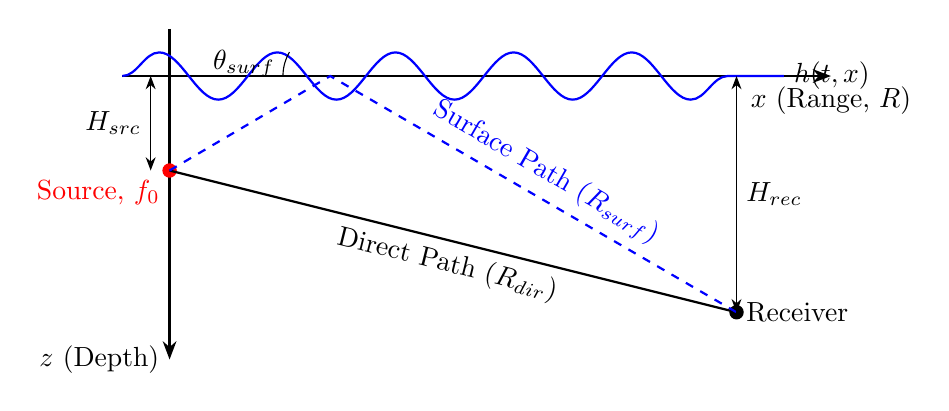
\begin{tikzpicture}[scale=1.2, >=Stealth]

    % Define variables/coordinates
    \def\Range{6}
    \def\Hrec{-2.5}
    \def\Hsrc{-1.0}
    
    % Draw axes
    \draw[->, thick] (0, 0.5) -- (0, \Hrec - 0.5) node[left] {$z$ (Depth)};
    \draw[->, thick] (-0.5, 0) -- (\Range + 1, 0) node[below] {$x$ (Range, $R$)};
    
    % Draw rough ocean surface
    \draw[blue, thick, decoration={snake, amplitude=3mm, segment length=15mm}, decorate] 
        (-0.5, 0) -- (\Range + 0.5, 0) node[right, text=black] {$h(t, x)$};
        
    % Underwater Source Vessel
    \filldraw[red] (0,\Hsrc) circle (2pt) node[below left] {Source, $f_0$};
    \draw[<->] (-0.2, 0) -- (-0.2, \Hsrc) node[midway, left] {$H_{src}$};
    
    % Receiver
    \filldraw[black] (\Range, \Hrec) circle (2pt) node[right] {Receiver};
    
    % Direct path
    \draw[solid, thick] (0,\Hsrc) -- (\Range, \Hrec) node[midway, below, sloped] {Direct Path ($R_{dir}$)};
    
    % Surface interaction path (Resolved Multipath)
    \draw[blue, dashed, thick] (0,\Hsrc) -- (1.7, 0) -- (\Range, \Hrec) node[midway, above, sloped, text=blue] {Surface Path ($R_{surf}$)};
    
    % Grazing Angle at surface
    \draw (1.2, 0) arc (180:{180+atan(\Hsrc/1.7)}:0.5) node[midway, left] {$\theta_{surf}$};
    
    % Annotate Depth and Range
    \draw[<->] (\Range, 0) -- (\Range, \Hrec) node[midway, right] {$H_{rec}$};
    
\end{tikzpicture}

\subsection{Physical \& Mathematical Breakdown}

When a vessel is submerged ($H_{src} \gg 0$), it is physically decoupled from the ocean's dynamic boundary. 
This decoupling mathematically breaks both the kinematic frequency modulation (FM) and the multiplicative micro-multipath fading.

\subsubsection{Elimination of Source Kinematics}

An underwater source operates below the wave base, meaning it is not subjected to the physical heave of the ocean swell.

The vertical heave amplitude approaches zero ($A_w \approx 0$).
Consequently, the Modulation Index ($\beta$) collapses:
\begin{equation}
\beta = \frac{2\pi f_0}{c} A_w \cos\theta_g \approx 0
\end{equation}

Applying $\beta = 0$ to the Jacobi-Anger expansion (the Bessel comb) yields $J_0(0) = 1$ and all higher-order Bessel functions $J_n(0) = 0$. The theoretical infinite bandwidth collapses back into a single singularity. The transmitted signal $p_{tx}(t)$ reverts entirely to a pure, unmodulated monochromatic wave:
\begin{equation}
p_{tx}(t) = P_0 \cos(2\pi f_0 t)
\end{equation}

meaning the source is emitting a theoretically perfect, infinitely narrow tonal.

\subsubsection{Resolution of Macro-Multipath}

For an underwater vessel, $H_{src}$ is a large, non-zero value. 
Because of this depth, the geometry creates a significant difference in path lengths:
\begin{equation}
R_{surf} \gg R_{dir}
\end{equation}

The time delay between the direct path and the surface echo becomes macroscopic ($\Delta \tau = \tau_{surf} - \tau_{dir} \gg 0$).

Because the signals no longer arrive at the same time, they can no longer interfere multiplicatively. 
The superposition equation is the sum of two separate, additive events in time.

\subsubsection{The Decoupled Received Signal}

Substituting our pure transmitted signal ($p_{tx}$) and our macro-delayed surface reflection into the receiver equation yields the theoretical received signal for an underwater vessel:
\begin{equation}
p_{rx}(t) = \underbrace{ \frac{P_0}{R_{dir}} \cos(2\pi f_0 (t - \tau_{dir})) }_{\text{Direct Path}} + \underbrace{ \frac{P_0 V(t)}{R_{surf}} \cos(2\pi f_0 (t - \tau_{surf})) }_{\text{Surface Echo}}
\end{equation}

This equation perfectly defines why the main signal is not smeared:
\begin{enumerate}
    \item \textbf{The Direct Path is Pristine:} is a perfect, time-delayed copy of the original engine tonal.
    \item \textbf{The Echo is Isolated:} the second term contains the time-varying scattering coefficient $V(t)$, which means the Doppler phase modulation from the moving surface does happen to the echo. However, because $\tau_{surf}$ is significantly larger than $\tau_{dir}$, it arrives much later.
    \item \textbf{Additive vs. Multiplicative:} the echo is temporally separated, it adds background reverberation (clutter) to the environment, but it does not multiplicatively modulate or fade the primary direct-path tonal.
\end{enumerate}

The geometry guarantees a pure, stable direct path that is mathematically independent of the surface dynamics. The surface smearing still exists in the environment, but it is confined entirely to a delayed, isolated echo, leaving the primary mechanical tonal sharp and un-smeared.


\clearpage
\section{Flow Diagram}

\resizebox{\textwidth}{!}{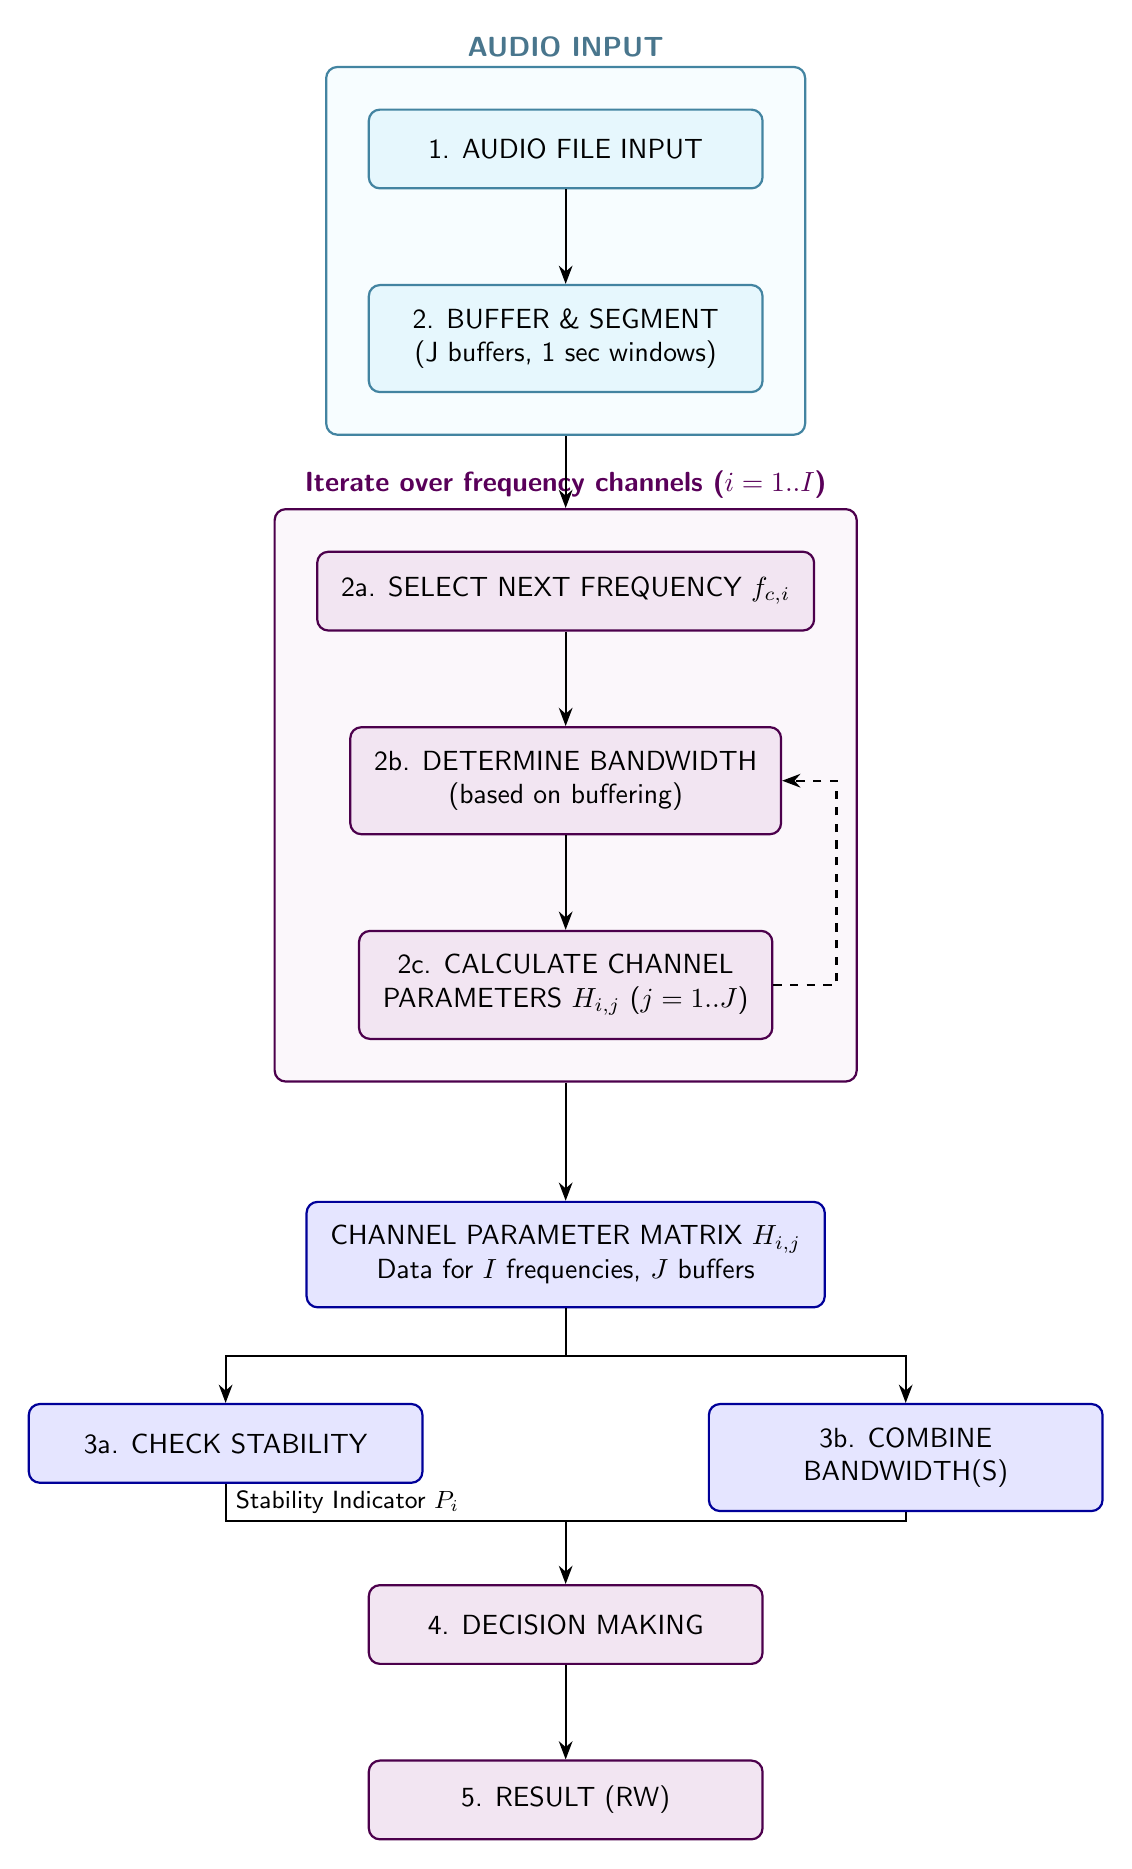
\begin{tikzpicture}[
    >=Stealth,
    node distance=1.2cm and 1.5cm,
    font=\sffamily,
    % Define styles for the different node types
    cyanbox/.style={rectangle, rounded corners, draw=cyan!60!black, fill=cyan!10, thick, text centered, align=center, minimum width=5cm, minimum height=1cm, inner sep=2ex},
    bluebox/.style={rectangle, rounded corners, draw=blue!60!black, fill=blue!10, thick, text centered, align=center, minimum width=5cm, minimum height=1cm, inner sep=2ex},
    purplebox/.style={rectangle, rounded corners, draw=violet!60!black, fill=violet!10, thick, text centered, align=center, minimum width=5cm, minimum height=1cm, inner sep=2ex},
    greenbox/.style={rectangle, rounded corners, draw=green!50!black, fill=green!10, thick, text centered, align=center, minimum height=0.8cm, inner sep=1.5ex},
    cyancontainer/.style={rectangle, rounded corners, draw=cyan!60!black, fill=cyan!3, thick, inner sep=15pt},
    purplecontainer/.style={rectangle, rounded corners, draw=violet!60!black, fill=violet!3, thick, inner sep=15pt},
]

% -------------------------
% Main Flow Nodes
% -------------------------
\node (audio) [cyanbox] {1. AUDIO FILE INPUT};
\node (buffer) [cyanbox, below=of audio] {2. BUFFER \& SEGMENT\\(J buffers, 1 sec windows)};

% Loop Inner Nodes
\node (c1) [purplebox, below=2cm of buffer] {2a. SELECT NEXT FREQUENCY $f_{c,i}$};
\node (c2) [purplebox, below=of c1] {2b. DETERMINE BANDWIDTH\\(based on buffering)};
\node (c3) [purplebox, below=of c2] {2c. CALCULATE CHANNEL\\PARAMETERS $H_{i,j}$ ($j=1..J$)};

% Loop Container Box
\begin{scope}[on background layer]
    \node (loopgroup) [purplecontainer, fit=(c1) (c2) (c3), label={[font=\sffamily\bfseries, text=violet!70!black]above:Iterate over frequency channels ($i=1..I$)}] {};
\end{scope}

\node (matrix) [bluebox, below=1.5cm of loopgroup] {CHANNEL PARAMETER MATRIX $H_{i,j}$\\Data for $I$ frequencies, $J$ buffers};

% Split Output Nodes
\node (stability) [bluebox, below left=1.2cm and -1.5cm of matrix] {3a. CHECK STABILITY};
\node (combine) [bluebox, below right=1.2cm and -1.5cm of matrix] {3b. COMBINE\\BANDWIDTH(S)};

% Final Nodes
\node (decision) [purplebox, below=3.5cm of matrix] {4. DECISION MAKING};
\node (result) [purplebox, below=of decision] {5. RESULT (RW)};


% Audio Input Container Box
\begin{scope}[on background layer]
    \node (inputgroup) [cyancontainer, fit=(audio) (buffer), label={[font=\sffamily\bfseries, text=cyan!50!black]above:AUDIO INPUT}] {};
\end{scope}


% -------------------------
% Arrow Connections
% -------------------------

% Input group to loop group
\draw[->, thick] (inputgroup.south) -- (loopgroup.north);

% Main flow top
\draw[->, thick] (audio) -- (buffer);

% Loop internals
\draw[->, thick] (c1) -- (c2);
\draw[->, thick] (c2) -- (c3);
% Feedback loop (dashed)
\draw[->, thick, dashed] (c3.east) -- ++(0.8,0) |- (c2.east);

% Loop to matrix
\draw[->, thick] (loopgroup.south) -- (matrix.north);

% Matrix to Split
\coordinate (matrix_split) at ($(matrix.south) + (0,-0.6)$);
\draw[thick] (matrix.south) -- (matrix_split);
\draw[->, thick] (matrix_split) -| (stability.north);
\draw[->, thick] (matrix_split) -| (combine.north);

% Split to Decision
\coordinate (decision_merge) at ($(decision.north) + (0,0.8)$);
\draw[thick] (stability.south) |- (decision_merge) node[near start, right, font=\sffamily\small] {Stability Indicator $P_i$};
\draw[thick] (combine.south) |- (decision_merge);
\draw[->, thick] (decision_merge) -- (decision.north);

% Decision to Result
\draw[->, thick] (decision) -- (result);

\end{tikzpicture}}

\begin{thebibliography}{9}
\bibitem{stojanovic1996recent}
M.~Stojanovic, ``Recent advances in high-speed underwater acoustic communications,'' \emph{IEEE Journal of Oceanic Engineering}, vol.~21, no.~2, pp. 125--136, 1996.

\bibitem{preisig2007acoustic}
J.~C. Preisig, ``Acoustic propagation considerations for underwater acoustic communications,'' \emph{IEEE Communications Magazine}, vol.~45, no.~12, pp. 110--117, 2007.

\bibitem{carlson2001}
A.~B. Carlson, P.~B. Crilly, and J.~C. Rutledge, \emph{Communication Systems: An Introduction to Signals and Noise in Electrical Communication}, 4th~ed.\hskip 1em plus 0.5em minus 0.4em\relax McGraw-Hill, 2001.

\bibitem{bass1979wave}
F.~G. Bass and I.~M. Fuks, \emph{Wave Scattering from Statistically Rough Surfaces}.\hskip 1em plus 0.5em minus 0.4em\relax Pergamon Press, Oxford, 1979.

\bibitem{roderick1979doppler}
W.~I. Roderick, ``Doppler spectra of acoustic signals reflected from a moving rough sea surface,'' Ph.D. dissertation, Yale University, New Haven, CT, 1979.
\end{thebibliography}

\end{document}